\documentclass[twoside]{book}

% Packages required by doxygen
\usepackage{calc}
\usepackage{doxygen}
\usepackage{graphicx}
\usepackage[utf8]{inputenc}
\usepackage{makeidx}
\usepackage{multicol}
\usepackage{multirow}
\usepackage{textcomp}
\usepackage[table]{xcolor}

% Font selection
\usepackage[T1]{fontenc}
\usepackage{mathptmx}
\usepackage[scaled=.90]{helvet}
\usepackage{courier}
\usepackage{amssymb}
\usepackage{sectsty}
\renewcommand{\familydefault}{\sfdefault}
\allsectionsfont{%
  \fontseries{bc}\selectfont%
  \color{darkgray}%
}
\renewcommand{\DoxyLabelFont}{%
  \fontseries{bc}\selectfont%
  \color{darkgray}%
}

% Page & text layout
\usepackage{geometry}
\geometry{%
  a4paper,%
  top=2.5cm,%
  bottom=2.5cm,%
  left=2.5cm,%
  right=2.5cm%
}
\tolerance=750
\hfuzz=15pt
\hbadness=750
\setlength{\emergencystretch}{15pt}
\setlength{\parindent}{0cm}
\setlength{\parskip}{0.2cm}
\makeatletter
\renewcommand{\paragraph}{%
  \@startsection{paragraph}{4}{0ex}{-1.0ex}{1.0ex}{%
    \normalfont\normalsize\bfseries\SS@parafont%
  }%
}
\renewcommand{\subparagraph}{%
  \@startsection{subparagraph}{5}{0ex}{-1.0ex}{1.0ex}{%
    \normalfont\normalsize\bfseries\SS@subparafont%
  }%
}
\makeatother

% Headers & footers
\usepackage{fancyhdr}
\pagestyle{fancyplain}
\fancyhead[LE]{\fancyplain{}{\bfseries\thepage}}
\fancyhead[CE]{\fancyplain{}{}}
\fancyhead[RE]{\fancyplain{}{\bfseries\leftmark}}
\fancyhead[LO]{\fancyplain{}{\bfseries\rightmark}}
\fancyhead[CO]{\fancyplain{}{}}
\fancyhead[RO]{\fancyplain{}{\bfseries\thepage}}
\fancyfoot[LE]{\fancyplain{}{}}
\fancyfoot[CE]{\fancyplain{}{}}
\fancyfoot[RE]{\fancyplain{}{\bfseries\scriptsize Generated on Sat Nov 16 2013 11\-:36\-:42 for My Project by Doxygen }}
\fancyfoot[LO]{\fancyplain{}{\bfseries\scriptsize Generated on Sat Nov 16 2013 11\-:36\-:42 for My Project by Doxygen }}
\fancyfoot[CO]{\fancyplain{}{}}
\fancyfoot[RO]{\fancyplain{}{}}
\renewcommand{\footrulewidth}{0.4pt}
\renewcommand{\chaptermark}[1]{%
  \markboth{#1}{}%
}
\renewcommand{\sectionmark}[1]{%
  \markright{\thesection\ #1}%
}

% Indices & bibliography
\usepackage{natbib}
\usepackage[titles]{tocloft}
\setcounter{tocdepth}{3}
\setcounter{secnumdepth}{5}
\makeindex

% Hyperlinks (required, but should be loaded last)
\usepackage{ifpdf}
\ifpdf
  \usepackage[pdftex,pagebackref=true]{hyperref}
\else
  \usepackage[ps2pdf,pagebackref=true]{hyperref}
\fi
\hypersetup{%
  colorlinks=true,%
  linkcolor=blue,%
  citecolor=blue,%
  unicode%
}

% Custom commands
\newcommand{\clearemptydoublepage}{%
  \newpage{\pagestyle{empty}\cleardoublepage}%
}


%===== C O N T E N T S =====

\begin{document}

% Titlepage & ToC
\hypersetup{pageanchor=false}
\pagenumbering{roman}
\begin{titlepage}
\vspace*{7cm}
\begin{center}%
{\Large My Project }\\
\vspace*{1cm}
{\large Generated by Doxygen 1.8.5}\\
\vspace*{0.5cm}
{\small Sat Nov 16 2013 11:36:42}\\
\end{center}
\end{titlepage}
\clearemptydoublepage
\tableofcontents
\clearemptydoublepage
\pagenumbering{arabic}
\hypersetup{pageanchor=true}

%--- Begin generated contents ---
\chapter{Hierarchical Index}
\section{Class Hierarchy}
This inheritance list is sorted roughly, but not completely, alphabetically\-:\begin{DoxyCompactList}
\item Mouse\-Listener\begin{DoxyCompactList}
\item \contentsline{section}{Image\-Pane}{\pageref{class_image_pane}}{}
\end{DoxyCompactList}
\item Mouse\-Motion\-Listener\begin{DoxyCompactList}
\item \contentsline{section}{Image\-Pane}{\pageref{class_image_pane}}{}
\end{DoxyCompactList}
\item \contentsline{section}{Photo}{\pageref{class_photo}}{}
\item \contentsline{section}{Photo\-Directory}{\pageref{class_photo_directory}}{}
\item \contentsline{section}{Photo\-List}{\pageref{class_photo_list}}{}
\item Action\-Listener\begin{DoxyCompactList}
\item \contentsline{section}{Control\-Pane}{\pageref{class_control_pane}}{}
\end{DoxyCompactList}
\item File\-Filter\begin{DoxyCompactList}
\item \contentsline{section}{Photo\-List.\-Image\-File\-Filter}{\pageref{class_photo_list_1_1_image_file_filter}}{}
\end{DoxyCompactList}
\item Focus\-Listener\begin{DoxyCompactList}
\item \contentsline{section}{Control\-Pane}{\pageref{class_control_pane}}{}
\end{DoxyCompactList}
\item J\-Frame\begin{DoxyCompactList}
\item \contentsline{section}{Folder\-G\-U\-I}{\pageref{class_folder_g_u_i}}{}
\item \contentsline{section}{Viewer\-G\-U\-I}{\pageref{class_viewer_g_u_i}}{}
\end{DoxyCompactList}
\item J\-Panel\begin{DoxyCompactList}
\item \contentsline{section}{Control\-Pane}{\pageref{class_control_pane}}{}
\item \contentsline{section}{Image\-Pane}{\pageref{class_image_pane}}{}
\end{DoxyCompactList}
\end{DoxyCompactList}

\chapter{Class Index}
\section{Class List}
Here are the classes, structs, unions and interfaces with brief descriptions\-:\begin{DoxyCompactList}
\item\contentsline{section}{\hyperlink{class_control_pane}{Control\-Pane} }{\pageref{class_control_pane}}{}
\item\contentsline{section}{\hyperlink{class_folder_g_u_i}{Folder\-G\-U\-I} }{\pageref{class_folder_g_u_i}}{}
\item\contentsline{section}{\hyperlink{class_photo_list_1_1_image_file_filter}{Photo\-List.\-Image\-File\-Filter} }{\pageref{class_photo_list_1_1_image_file_filter}}{}
\item\contentsline{section}{\hyperlink{class_image_pane}{Image\-Pane} }{\pageref{class_image_pane}}{}
\item\contentsline{section}{\hyperlink{class_photo}{Photo} }{\pageref{class_photo}}{}
\item\contentsline{section}{\hyperlink{class_photo_directory}{Photo\-Directory} }{\pageref{class_photo_directory}}{}
\item\contentsline{section}{\hyperlink{class_photo_list}{Photo\-List} }{\pageref{class_photo_list}}{}
\item\contentsline{section}{\hyperlink{class_viewer_g_u_i}{Viewer\-G\-U\-I} }{\pageref{class_viewer_g_u_i}}{}
\end{DoxyCompactList}

\chapter{Class Documentation}
\hypertarget{class_control_pane}{\section{Control\-Pane Class Reference}
\label{class_control_pane}\index{Control\-Pane@{Control\-Pane}}
}


Inheritance diagram for Control\-Pane\-:
\nopagebreak
\begin{figure}[H]
\begin{center}
\leavevmode
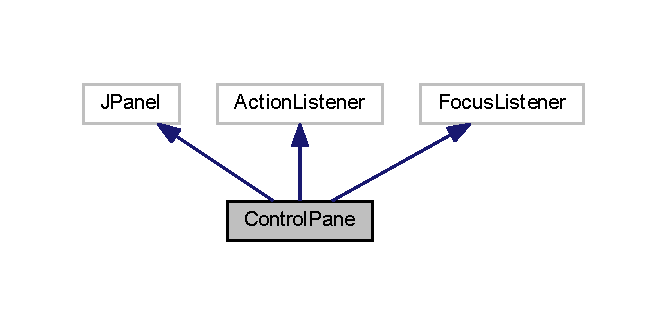
\includegraphics[width=320pt]{class_control_pane__inherit__graph}
\end{center}
\end{figure}


Collaboration diagram for Control\-Pane\-:
\nopagebreak
\begin{figure}[H]
\begin{center}
\leavevmode
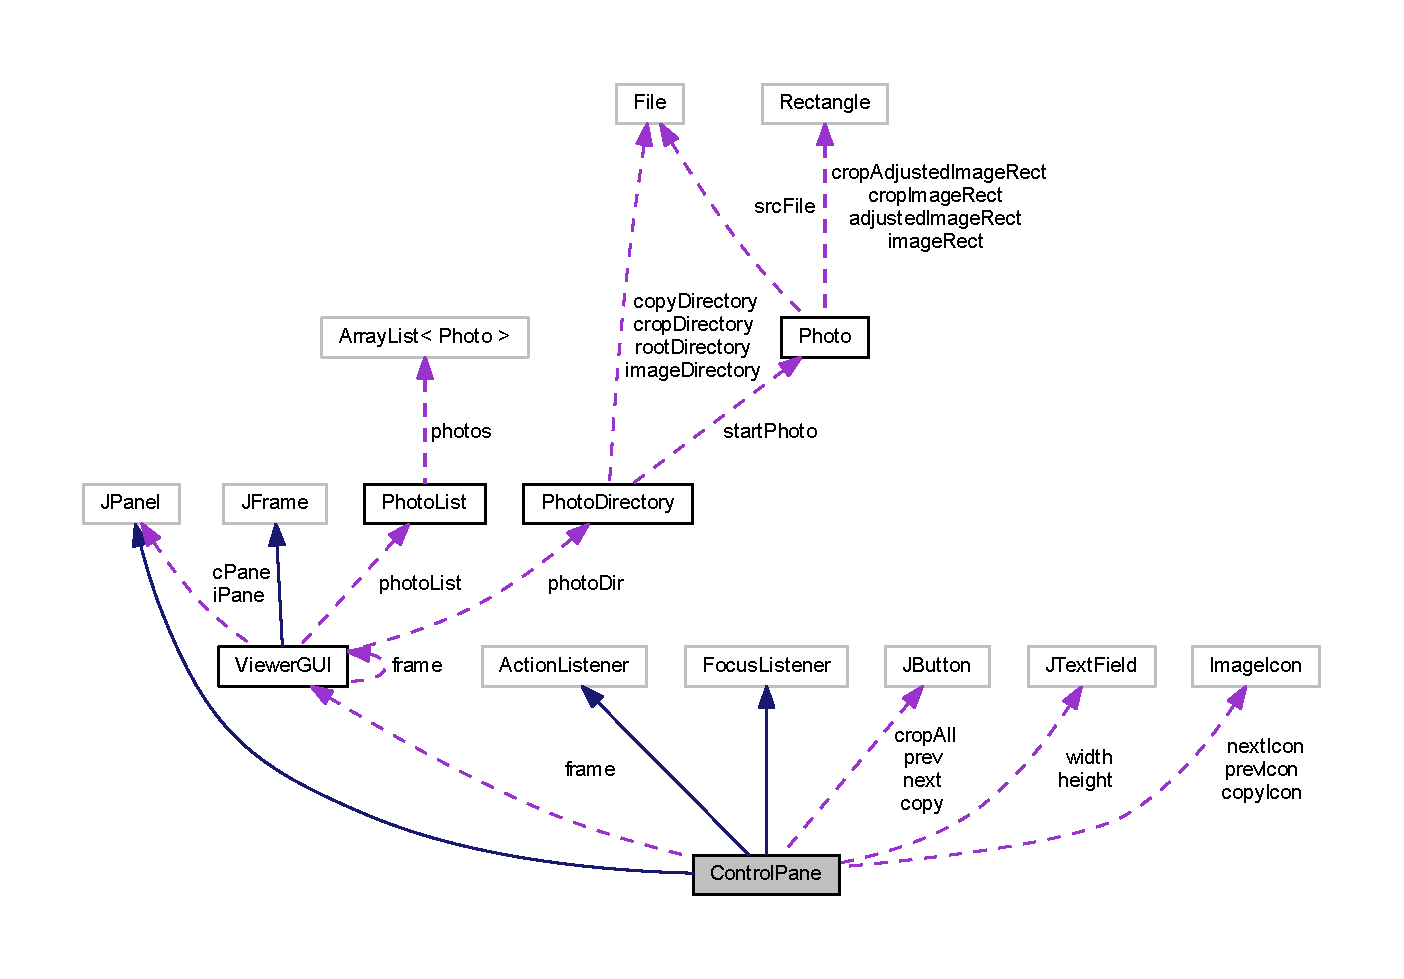
\includegraphics[width=350pt]{class_control_pane__coll__graph}
\end{center}
\end{figure}
\subsection*{Public Member Functions}
\begin{DoxyCompactItemize}
\item 
\hypertarget{class_control_pane_a1c330f498e14b6054709854eaec034c9}{{\bfseries Control\-Pane} (\hyperlink{class_viewer_g_u_i}{Viewer\-G\-U\-I} parent)}\label{class_control_pane_a1c330f498e14b6054709854eaec034c9}

\item 
\hypertarget{class_control_pane_af35ca5536e4b94d83dd308b97eaa9b7b}{void {\bfseries action\-Performed} (Action\-Event e)}\label{class_control_pane_af35ca5536e4b94d83dd308b97eaa9b7b}

\item 
\hypertarget{class_control_pane_a2994c5fed9033e309f4e1efa18a77a29}{void {\bfseries focus\-Gained} (Focus\-Event e)}\label{class_control_pane_a2994c5fed9033e309f4e1efa18a77a29}

\item 
\hypertarget{class_control_pane_a26ae6778853f590a9e501f759cce3f13}{void {\bfseries focus\-Lost} (Focus\-Event e)}\label{class_control_pane_a26ae6778853f590a9e501f759cce3f13}

\end{DoxyCompactItemize}


The documentation for this class was generated from the following file\-:\begin{DoxyCompactItemize}
\item 
Control\-Pane.\-java\end{DoxyCompactItemize}

\hypertarget{class_folder_g_u_i}{\section{Folder\-G\-U\-I Class Reference}
\label{class_folder_g_u_i}\index{Folder\-G\-U\-I@{Folder\-G\-U\-I}}
}


Inheritance diagram for Folder\-G\-U\-I\-:
\nopagebreak
\begin{figure}[H]
\begin{center}
\leavevmode
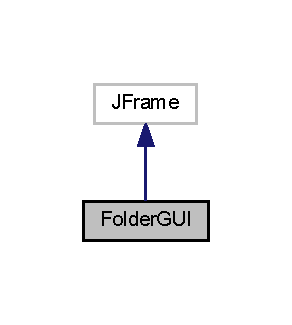
\includegraphics[width=140pt]{class_folder_g_u_i__inherit__graph}
\end{center}
\end{figure}


Collaboration diagram for Folder\-G\-U\-I\-:
\nopagebreak
\begin{figure}[H]
\begin{center}
\leavevmode
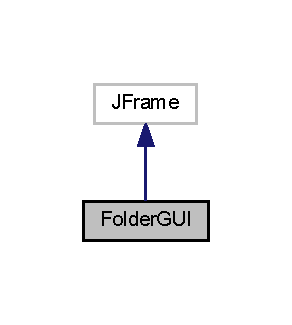
\includegraphics[width=140pt]{class_folder_g_u_i__coll__graph}
\end{center}
\end{figure}


The documentation for this class was generated from the following file\-:\begin{DoxyCompactItemize}
\item 
Folder\-G\-U\-I.\-java\end{DoxyCompactItemize}

\hypertarget{class_photo_list_1_1_image_file_filter}{\section{Photo\-List.\-Image\-File\-Filter Class Reference}
\label{class_photo_list_1_1_image_file_filter}\index{Photo\-List.\-Image\-File\-Filter@{Photo\-List.\-Image\-File\-Filter}}
}


Inheritance diagram for Photo\-List.\-Image\-File\-Filter\-:
\nopagebreak
\begin{figure}[H]
\begin{center}
\leavevmode
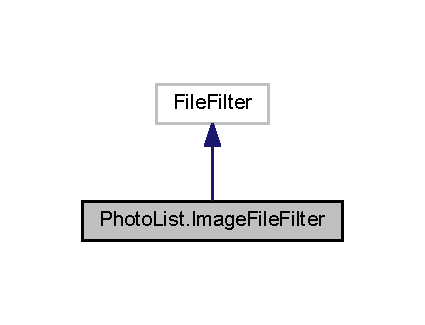
\includegraphics[width=204pt]{class_photo_list_1_1_image_file_filter__inherit__graph}
\end{center}
\end{figure}


Collaboration diagram for Photo\-List.\-Image\-File\-Filter\-:
\nopagebreak
\begin{figure}[H]
\begin{center}
\leavevmode
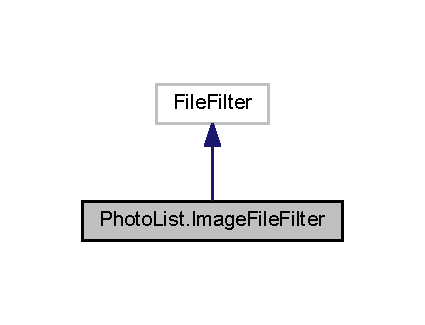
\includegraphics[width=204pt]{class_photo_list_1_1_image_file_filter__coll__graph}
\end{center}
\end{figure}
\subsection*{Public Member Functions}
\begin{DoxyCompactItemize}
\item 
\hypertarget{class_photo_list_1_1_image_file_filter_a3e44844354fe08b8ae7d2e2a35c695c3}{boolean {\bfseries accept} (File file)}\label{class_photo_list_1_1_image_file_filter_a3e44844354fe08b8ae7d2e2a35c695c3}

\end{DoxyCompactItemize}


The documentation for this class was generated from the following file\-:\begin{DoxyCompactItemize}
\item 
Photo\-List.\-java\end{DoxyCompactItemize}

\hypertarget{class_image_pane}{\section{Image\-Pane Class Reference}
\label{class_image_pane}\index{Image\-Pane@{Image\-Pane}}
}


Inheritance diagram for Image\-Pane\-:
\nopagebreak
\begin{figure}[H]
\begin{center}
\leavevmode
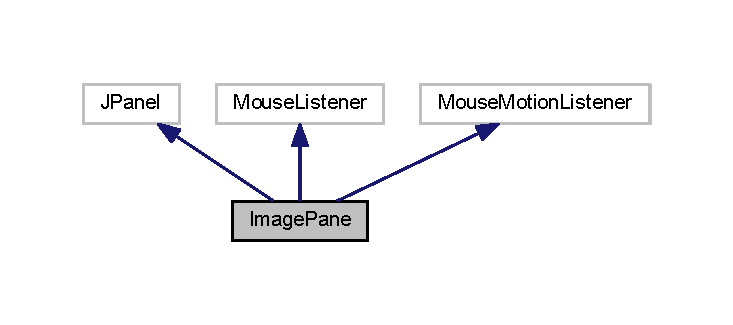
\includegraphics[width=350pt]{class_image_pane__inherit__graph}
\end{center}
\end{figure}


Collaboration diagram for Image\-Pane\-:
\nopagebreak
\begin{figure}[H]
\begin{center}
\leavevmode
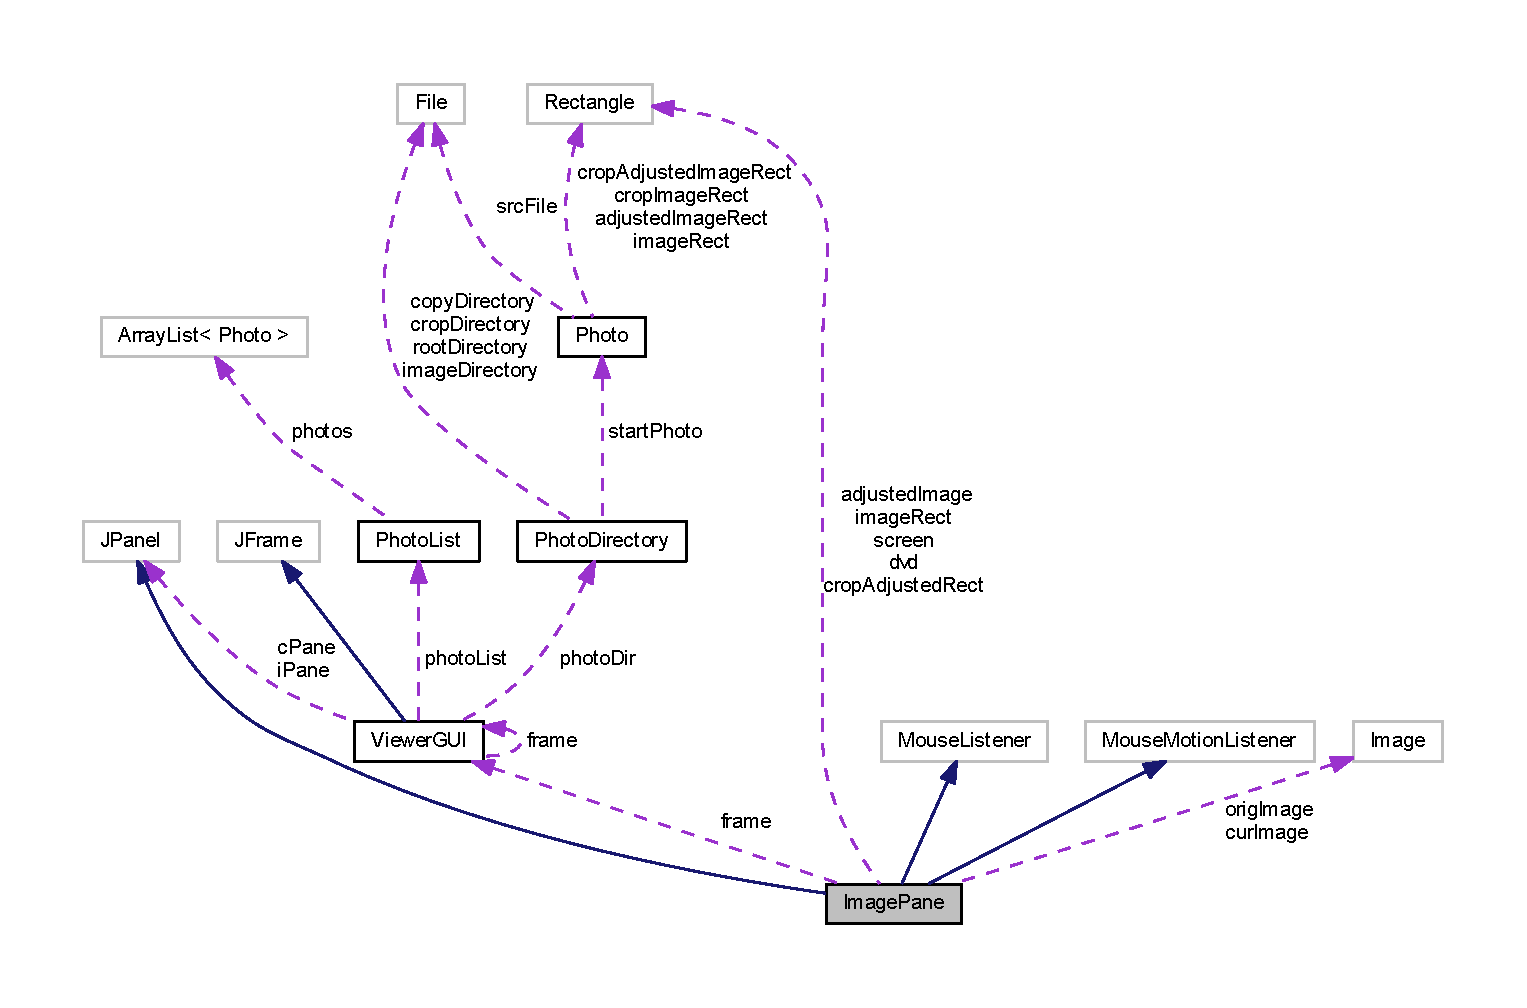
\includegraphics[width=350pt]{class_image_pane__coll__graph}
\end{center}
\end{figure}
\subsection*{Public Member Functions}
\begin{DoxyCompactItemize}
\item 
\hypertarget{class_image_pane_a255cfe2fc340af5859f8862e56fe54be}{boolean {\bfseries get\-Crop\-Flag} ()}\label{class_image_pane_a255cfe2fc340af5859f8862e56fe54be}

\item 
\hypertarget{class_image_pane_a5c2576cd6c9aa7748e3cb9733a03f29c}{boolean {\bfseries get\-Cropped\-All\-Flag} ()}\label{class_image_pane_a5c2576cd6c9aa7748e3cb9733a03f29c}

\item 
\hypertarget{class_image_pane_ade727efbec66dddd425374b7c6a207ba}{void {\bfseries set\-Dvd\-Width} (int w)}\label{class_image_pane_ade727efbec66dddd425374b7c6a207ba}

\item 
\hypertarget{class_image_pane_a201e6feac95148c9734a530b98d9e9a5}{void {\bfseries set\-Dvd\-Height} (int h)}\label{class_image_pane_a201e6feac95148c9734a530b98d9e9a5}

\item 
\hypertarget{class_image_pane_a198d4686ed7b1db5d87dd2982f606bd1}{void {\bfseries reset\-Dvd\-Width} ()}\label{class_image_pane_a198d4686ed7b1db5d87dd2982f606bd1}

\item 
\hypertarget{class_image_pane_a76a8b0ef65f6f0c0461ee6be1b68f619}{void {\bfseries reset\-Dvd\-Height} ()}\label{class_image_pane_a76a8b0ef65f6f0c0461ee6be1b68f619}

\item 
\hypertarget{class_image_pane_a3928985ebb14e16410e38e252dbefd05}{Rectangle {\bfseries get\-Crop\-Adjusted\-Rect} ()}\label{class_image_pane_a3928985ebb14e16410e38e252dbefd05}

\item 
\hypertarget{class_image_pane_af0d11a52742ce1884eedbfb6d3e3e97f}{Rectangle {\bfseries get\-Adjusted\-Image} ()}\label{class_image_pane_af0d11a52742ce1884eedbfb6d3e3e97f}

\item 
\hypertarget{class_image_pane_a396110fc43247e26bb0a61aad98e2244}{void {\bfseries set\-Crop\-Flag} (boolean flag)}\label{class_image_pane_a396110fc43247e26bb0a61aad98e2244}

\item 
\hypertarget{class_image_pane_a8ae8755a8ac3800eed97d9d5ffb78e0f}{void {\bfseries set\-Cropped\-All\-Flag} (boolean flag)}\label{class_image_pane_a8ae8755a8ac3800eed97d9d5ffb78e0f}

\item 
\hypertarget{class_image_pane_a370a844b6b3ca53f6f46c9bf9eacea0d}{{\bfseries Image\-Pane} (\hyperlink{class_viewer_g_u_i}{Viewer\-G\-U\-I} parent)  throws I\-O\-Exception}\label{class_image_pane_a370a844b6b3ca53f6f46c9bf9eacea0d}

\item 
\hypertarget{class_image_pane_a23cfe102398698d805849dae2ec47e5d}{void {\bfseries set\-Screen\-Image} (\hyperlink{class_photo}{Photo} photo)}\label{class_image_pane_a23cfe102398698d805849dae2ec47e5d}

\item 
\hypertarget{class_image_pane_a9ec3e046d345688f9a07f67ec71fedf2}{boolean {\bfseries image\-Update} (Image img, int infoflags, int x, int y, int width, int height)}\label{class_image_pane_a9ec3e046d345688f9a07f67ec71fedf2}

\item 
\hypertarget{class_image_pane_a88fe5d1f503edb079fa8dc14f222ac37}{void {\bfseries paint\-Component} (Graphics g)}\label{class_image_pane_a88fe5d1f503edb079fa8dc14f222ac37}

\item 
\hypertarget{class_image_pane_a3121ca3a794eed6b5cd5248e05ffdc0f}{void {\bfseries mouse\-Moved} (Mouse\-Event arg0)}\label{class_image_pane_a3121ca3a794eed6b5cd5248e05ffdc0f}

\item 
\hypertarget{class_image_pane_a73e8b977b5d37689b78b75ef58ed7586}{void {\bfseries mouse\-Clicked} (Mouse\-Event arg0)}\label{class_image_pane_a73e8b977b5d37689b78b75ef58ed7586}

\item 
\hypertarget{class_image_pane_ac1598e74cca9e8705a1fab96c67210ce}{void {\bfseries mouse\-Entered} (Mouse\-Event arg0)}\label{class_image_pane_ac1598e74cca9e8705a1fab96c67210ce}

\item 
\hypertarget{class_image_pane_ae5fd189211613be83cc8e28000123c5c}{void {\bfseries mouse\-Exited} (Mouse\-Event arg0)}\label{class_image_pane_ae5fd189211613be83cc8e28000123c5c}

\item 
\hypertarget{class_image_pane_a448ca5113bef60eed8460be3a9451f11}{void {\bfseries mouse\-Pressed} (Mouse\-Event e)}\label{class_image_pane_a448ca5113bef60eed8460be3a9451f11}

\item 
\hypertarget{class_image_pane_adc4d5e86b56dab9fb6e8d37fcea5b239}{void {\bfseries mouse\-Released} (Mouse\-Event e)}\label{class_image_pane_adc4d5e86b56dab9fb6e8d37fcea5b239}

\item 
\hypertarget{class_image_pane_af6f08d292b6fdf7ca49bbedff10a1965}{void {\bfseries mouse\-Dragged} (Mouse\-Event e)}\label{class_image_pane_af6f08d292b6fdf7ca49bbedff10a1965}

\end{DoxyCompactItemize}


The documentation for this class was generated from the following file\-:\begin{DoxyCompactItemize}
\item 
Image\-Pane.\-java\end{DoxyCompactItemize}

\hypertarget{class_photo}{\section{Photo Class Reference}
\label{class_photo}\index{Photo@{Photo}}
}


Collaboration diagram for Photo\-:
\nopagebreak
\begin{figure}[H]
\begin{center}
\leavevmode
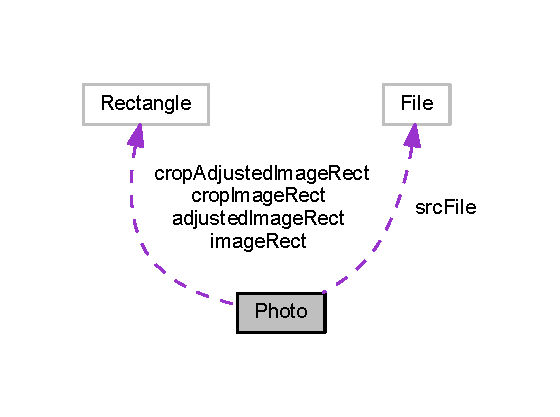
\includegraphics[width=269pt]{class_photo__coll__graph}
\end{center}
\end{figure}
\subsection*{Public Member Functions}
\begin{DoxyCompactItemize}
\item 
\hypertarget{class_photo_a34fb5fcdc854bddfe5bcaf52fc4bedc9}{{\bfseries Photo} (File s\-File)}\label{class_photo_a34fb5fcdc854bddfe5bcaf52fc4bedc9}

\item 
\hypertarget{class_photo_a9fc3e7f49ec338b2097baf8c02277e3a}{{\bfseries Photo} (File src\-File, Rectangle src\-Crop)}\label{class_photo_a9fc3e7f49ec338b2097baf8c02277e3a}

\item 
\hypertarget{class_photo_a2ead9b28a76e7969b940fd0bc0df2eb7}{String {\bfseries get\-Name} ()}\label{class_photo_a2ead9b28a76e7969b940fd0bc0df2eb7}

\item 
\hypertarget{class_photo_a27d5af5113f75e353b09c55242db79a7}{File {\bfseries get\-Src\-File} ()}\label{class_photo_a27d5af5113f75e353b09c55242db79a7}

\item 
\hypertarget{class_photo_aa0fe056b7b47f7d185dfe1ef33605933}{Image {\bfseries get\-Image} ()}\label{class_photo_aa0fe056b7b47f7d185dfe1ef33605933}

\item 
\hypertarget{class_photo_af19f3636644e6e4096abe161373ed86b}{Rectangle {\bfseries get\-Image\-Rect} ()}\label{class_photo_af19f3636644e6e4096abe161373ed86b}

\item 
\hypertarget{class_photo_afca1360208ac74f21156c30540358b07}{Rectangle {\bfseries get\-Crop\-Image\-Rect} ()}\label{class_photo_afca1360208ac74f21156c30540358b07}

\item 
\hypertarget{class_photo_a06bdd8ad343d72ed52b0788c0c14f5d4}{Rectangle {\bfseries get\-Crop\-Adjusted\-Image\-Rect} ()}\label{class_photo_a06bdd8ad343d72ed52b0788c0c14f5d4}

\item 
\hypertarget{class_photo_ad7f11dfd91805884d3210ae5a0a3d89c}{Rectangle {\bfseries get\-Adjusted\-Image\-Rect} ()}\label{class_photo_ad7f11dfd91805884d3210ae5a0a3d89c}

\item 
\hypertarget{class_photo_a779642ff1fa78ae161fd938a45d4ef77}{void {\bfseries set\-Image\-Rect} (int width, int height)}\label{class_photo_a779642ff1fa78ae161fd938a45d4ef77}

\item 
\hypertarget{class_photo_aa7a53aad4146948df48ac73e25ee9ebd}{void {\bfseries set\-Crop\-Image\-Rect} (Rectangle c\-Rect)}\label{class_photo_aa7a53aad4146948df48ac73e25ee9ebd}

\item 
\hypertarget{class_photo_aacf719d5137e8693755d382b518401e3}{void {\bfseries set\-Crop\-Adjusted\-Image\-Rect} (Rectangle c\-Rect)}\label{class_photo_aacf719d5137e8693755d382b518401e3}

\item 
\hypertarget{class_photo_a43da5ba27fb5ab7c236f5c6befa8ee32}{void {\bfseries set\-Adjusted\-Image\-Rect} (Rectangle a\-Rect)}\label{class_photo_a43da5ba27fb5ab7c236f5c6befa8ee32}

\item 
\hypertarget{class_photo_a04d29772c91304ba57e083c0b7c3e5e1}{void {\bfseries copy\-Photo} (\hyperlink{class_photo_directory}{Photo\-Directory} photo\-Dir)  throws I\-O\-Exception }\label{class_photo_a04d29772c91304ba57e083c0b7c3e5e1}

\item 
\hypertarget{class_photo_ae9333b659600b85c69bfb0f1621c580e}{void {\bfseries crop\-Photo} (\hyperlink{class_viewer_g_u_i}{Viewer\-G\-U\-I} frame)  throws I\-O\-Exception }\label{class_photo_ae9333b659600b85c69bfb0f1621c580e}

\item 
\hypertarget{class_photo_ac635da00197d7b7d50517b8f0218c2be}{void {\bfseries print} ()}\label{class_photo_ac635da00197d7b7d50517b8f0218c2be}

\end{DoxyCompactItemize}


The documentation for this class was generated from the following file\-:\begin{DoxyCompactItemize}
\item 
Photo.\-java\end{DoxyCompactItemize}

\hypertarget{class_photo_directory}{\section{Photo\-Directory Class Reference}
\label{class_photo_directory}\index{Photo\-Directory@{Photo\-Directory}}
}


Collaboration diagram for Photo\-Directory\-:
\nopagebreak
\begin{figure}[H]
\begin{center}
\leavevmode
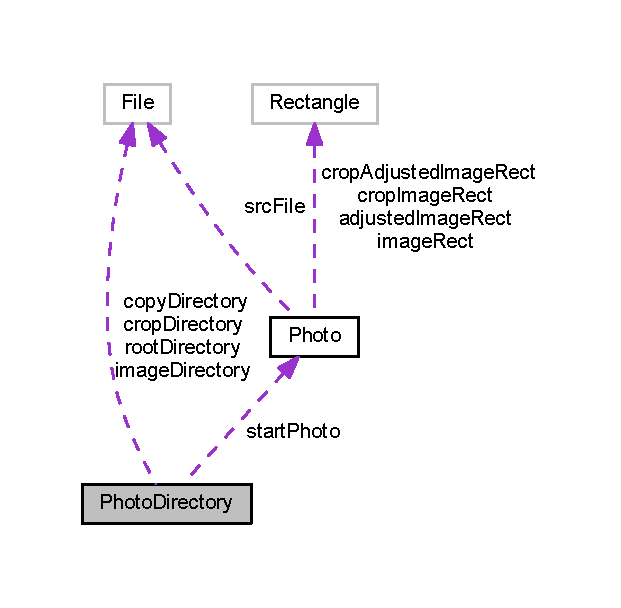
\includegraphics[width=298pt]{class_photo_directory__coll__graph}
\end{center}
\end{figure}
\subsection*{Public Member Functions}
\begin{DoxyCompactItemize}
\item 
\hypertarget{class_photo_directory_a9747fd41e2b47ec2af2a1335abb22255}{File {\bfseries get\-Image\-Directory} ()}\label{class_photo_directory_a9747fd41e2b47ec2af2a1335abb22255}

\item 
\hypertarget{class_photo_directory_a52c74f7d9f5ad19f8e8ec4f87339cdff}{File {\bfseries get\-Copy\-Directory} ()}\label{class_photo_directory_a52c74f7d9f5ad19f8e8ec4f87339cdff}

\item 
\hypertarget{class_photo_directory_a529f7fe8c7f74db920c783a07f427eb9}{File {\bfseries get\-Crop\-Directory} ()}\label{class_photo_directory_a529f7fe8c7f74db920c783a07f427eb9}

\item 
\hypertarget{class_photo_directory_a63de251b82177b9f68b9804ae548569d}{File {\bfseries get\-Root\-Directory} ()}\label{class_photo_directory_a63de251b82177b9f68b9804ae548569d}

\item 
\hypertarget{class_photo_directory_a6f069dd0739960d9654a80fd977ddbfd}{\hyperlink{class_photo}{Photo} {\bfseries get\-Start\-Photo} ()}\label{class_photo_directory_a6f069dd0739960d9654a80fd977ddbfd}

\item 
\hypertarget{class_photo_directory_aeed775d22ac8ef9319ff97b8212b78bf}{void {\bfseries setup\-Directories} (File image\-Dir, File start\-File)}\label{class_photo_directory_aeed775d22ac8ef9319ff97b8212b78bf}

\end{DoxyCompactItemize}


The documentation for this class was generated from the following file\-:\begin{DoxyCompactItemize}
\item 
Photo\-Directory.\-java\end{DoxyCompactItemize}

\hypertarget{class_photo_list}{\section{Photo\-List Class Reference}
\label{class_photo_list}\index{Photo\-List@{Photo\-List}}
}


Collaboration diagram for Photo\-List\-:
\nopagebreak
\begin{figure}[H]
\begin{center}
\leavevmode
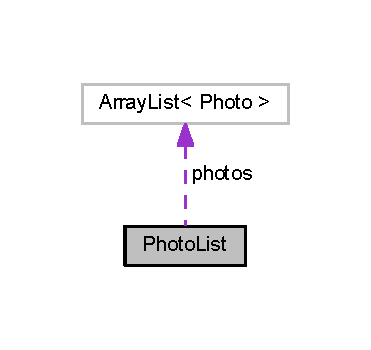
\includegraphics[width=178pt]{class_photo_list__coll__graph}
\end{center}
\end{figure}
\subsection*{Classes}
\begin{DoxyCompactItemize}
\item 
class \hyperlink{class_photo_list_1_1_image_file_filter}{Image\-File\-Filter}
\end{DoxyCompactItemize}
\subsection*{Public Member Functions}
\begin{DoxyCompactItemize}
\item 
\hypertarget{class_photo_list_ae628386e5f7f4674fc3426ff1b093c26}{\hyperlink{class_photo}{Photo} {\bfseries get\-Photo} ()}\label{class_photo_list_ae628386e5f7f4674fc3426ff1b093c26}

\item 
\hypertarget{class_photo_list_ac03d1e4822c26e086d9f6579be8f569f}{\hyperlink{class_photo}{Photo} {\bfseries get\-First\-Photo} ()}\label{class_photo_list_ac03d1e4822c26e086d9f6579be8f569f}

\item 
\hypertarget{class_photo_list_a9ca62869a8b779bd7fedad12362127e8}{\hyperlink{class_photo}{Photo} {\bfseries get\-Next\-Photo} ()}\label{class_photo_list_a9ca62869a8b779bd7fedad12362127e8}

\item 
\hypertarget{class_photo_list_afd0bcbf4fd13fa2a8408a649d56c6c8d}{\hyperlink{class_photo}{Photo} {\bfseries get\-Prev\-Photo} ()}\label{class_photo_list_afd0bcbf4fd13fa2a8408a649d56c6c8d}

\item 
\hypertarget{class_photo_list_ad1fe39413e463e258fc7cff2fcc7495e}{boolean {\bfseries at\-Beginning} ()}\label{class_photo_list_ad1fe39413e463e258fc7cff2fcc7495e}

\item 
\hypertarget{class_photo_list_a53fc4e93a8da830f3e8181e6853a22fa}{boolean {\bfseries at\-End} ()}\label{class_photo_list_a53fc4e93a8da830f3e8181e6853a22fa}

\item 
\hypertarget{class_photo_list_aa90131f591a2bc298254830b729ae82a}{void {\bfseries set\-Start\-Photo} (\hyperlink{class_photo}{Photo} photo)}\label{class_photo_list_aa90131f591a2bc298254830b729ae82a}

\item 
\hypertarget{class_photo_list_a63cf56455a46cdeb64ebfcb4797cfa01}{void {\bfseries load\-Images} (\hyperlink{class_photo_directory}{Photo\-Directory} photo\-Dir)}\label{class_photo_list_a63cf56455a46cdeb64ebfcb4797cfa01}

\item 
\hypertarget{class_photo_list_a4af932149cf1650bb5760a0c13d761f2}{void {\bfseries crop\-Photos} (\hyperlink{class_viewer_g_u_i}{Viewer\-G\-U\-I} frame)}\label{class_photo_list_a4af932149cf1650bb5760a0c13d761f2}

\item 
\hypertarget{class_photo_list_ab9c38b41e3a6d93bf524bc63fc254ea5}{void {\bfseries print\-Photos} ()}\label{class_photo_list_ab9c38b41e3a6d93bf524bc63fc254ea5}

\end{DoxyCompactItemize}


The documentation for this class was generated from the following file\-:\begin{DoxyCompactItemize}
\item 
Photo\-List.\-java\end{DoxyCompactItemize}

\hypertarget{class_viewer_g_u_i}{\section{Viewer\-G\-U\-I Class Reference}
\label{class_viewer_g_u_i}\index{Viewer\-G\-U\-I@{Viewer\-G\-U\-I}}
}


Inheritance diagram for Viewer\-G\-U\-I\-:
\nopagebreak
\begin{figure}[H]
\begin{center}
\leavevmode
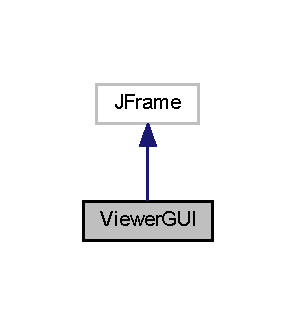
\includegraphics[width=142pt]{class_viewer_g_u_i__inherit__graph}
\end{center}
\end{figure}


Collaboration diagram for Viewer\-G\-U\-I\-:
\nopagebreak
\begin{figure}[H]
\begin{center}
\leavevmode
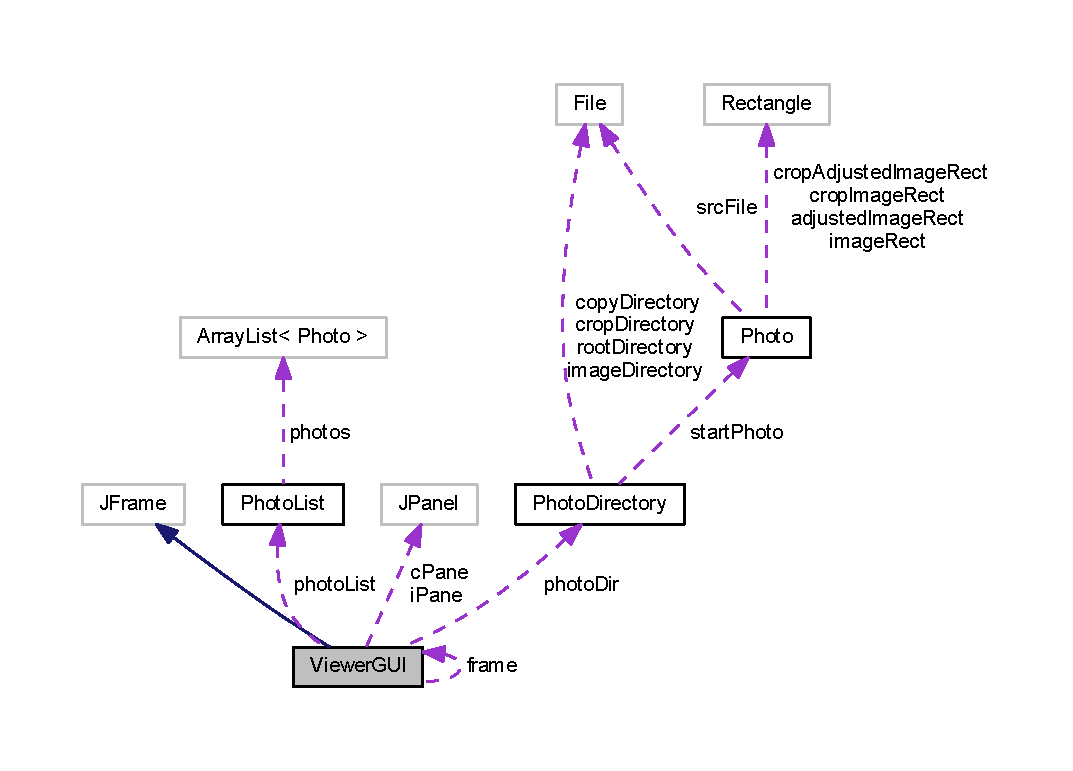
\includegraphics[width=350pt]{class_viewer_g_u_i__coll__graph}
\end{center}
\end{figure}
\subsection*{Static Public Member Functions}
\begin{DoxyCompactItemize}
\item 
\hypertarget{class_viewer_g_u_i_a688485c431b6d34895a9958cc2ae57f0}{static void {\bfseries main} (String\mbox{[}$\,$\mbox{]} arguments)  throws I\-O\-Exception }\label{class_viewer_g_u_i_a688485c431b6d34895a9958cc2ae57f0}

\end{DoxyCompactItemize}


The documentation for this class was generated from the following file\-:\begin{DoxyCompactItemize}
\item 
Viewer\-G\-U\-I.\-java\end{DoxyCompactItemize}

%--- End generated contents ---

% Index
\newpage
\phantomsection
\addcontentsline{toc}{part}{Index}
\printindex

\end{document}
